\documentclass[11pt, A4paper,norsk]{article}
\usepackage[utf8]{inputenc}
\usepackage[T1]{fontenc}
\usepackage{babel}
\usepackage{amsmath}
\usepackage{amsfonts}
\usepackage{amsthm}
\usepackage[colorlinks]{hyperref}
\usepackage{listings}
\usepackage{color}
\usepackage{hyperref}
\usepackage{graphicx}
\usepackage{cite}

\definecolor{dkgreen}{rgb}{0,0.6,0}
\definecolor{gray}{rgb}{0.5,0.5,0.5}
\definecolor{daynineyellow}{rgb}{1.0,0.655,0.102}
\definecolor{url}{rgb}{0.1,0.1,0.4}

\lstset{frame=tb,
	language=Python,
	aboveskip=3mm,
	belowskip=3mm,
	showstringspaces=false,
	columns=flexible,
	basicstyle={\small\ttfamily},
	numbers=none,
	numberstyle=\tiny\color{gray},
	keywordstyle=\color{blue},
	commentstyle=\color{daynineyellow},
	stringstyle=\color{dkgreen},
	breaklines=true,
	breakatwhitespace=true,
	tabsize=3
}

\lstset{inputpath="C:/Users/Torstein/Documents/UiO/Mat1110/Python programmer"}
\hypersetup{colorlinks, urlcolor=url}

\author{Torstein Solheim Ølberg}
\title{Svar på Oblig nr.1 i Mat1110}

\begin{document}
\maketitle
	\begin{center}
\Large \textbf{Oppgaver}
	\end{center}
		\paragraph{1.}
			\subparagraph{a)}
				\begin{flushleft}
Finn en matrise $M$ slik at $$x_{n+1} = \frac{1}{2} M x_n \nonumber$$ \\
\vspace{1mm}
\textbf{Løsning:} \\
\vspace{1mm}
					\begin{align}
x_{n+1} = \frac{1}{2} M x_n \nonumber \\
\left( \begin{tabular}{ c }
1/2 x_n + 1/2 z_n \\
1/2 y_n + 1/2 x_n \\
1/2 z_n + 1/2 y_n
\end{tabular} \right)
= \frac{1}{2} M 
\left( \begin{tabular}{ c }
x_n \\
y_n \\
z_n
\end{tabular} \right) \nonumber \\
\frac{1}{2}
\left( \begin{tabular}{ c }
x_n + z_n \\
y_n + x_n \\
z_n + y_n
\end{tabular} \right)
 = \frac{1}{2}
\left( \begin{tabular}{ ccc }
1 & 0 & 1 \\
1 & 1 & 0 \\
0 & 1 & 1
\end{tabular} \right) 
\left( \begin{tabular}{ c }
x_n \\
y_n \\
z_n
\end{tabular} \right) \nonumber
					\end{align}
				\end{flushleft}










			\subparagraph{b)}
				\begin{flushleft}
Finn egenverdiene og de tilhørende egenvektorene til $M$. \\
\vspace{1mm}
\textbf{Løsning:} \\
\vspace{1mm}
					\begin{align}
det(\lambda I_3 - M) = 0 \nonumber \\
det \left( \begin{tabular}{ ccc }
\lambda - 1 & 0 & -1 \\
-1 & \lambda - 1 & 0 \\
0 & -1 &  \lambda - 1
\end{tabular} \right) = 0 \nonumber \\
\lambda^3 - 3 \lambda^2 + 3 \lambda = 2 \nonumber \\
\lambda = 2, \frac{1 + sqrt(3)i}{2}, \frac{1 - sqrt(3)i}{2} \nonumber \\
\text{Dette gir at for $2$ kan egenvektoren være en hvilken som helst vektor} \nonumber \\
\text{så lenge alle tre variablene x, y, y er like.} \nonumber \\
\text{For $\frac{1 + sqrt(3)i}{2}$ blir egenvektoren:} \nonumber \\
\left( \begin{tabular}{ c }
1 \\
(- 1 + sqrt(3)i)^2/4 \\
(- 1 + sqrt(3)i)/2
\end{tabular} \right) \nonumber \\
\text{Og for $\frac{1 - sqrt(3)i}{2}$ blir egenvektoren:} \nonumber \\
\left( \begin{tabular}{ c }
1 \\
(- 1 - sqrt(3)i)^2/4 \\
(- 1 - sqrt(3)i)/2
\end{tabular} \right) \nonumber
					\end{align}
Egenvektorene er regnet ut ved å bruke at $A \cdot v = \lambda \cdot v$ og velge $x = 1$ og regne ut de andre verdiene deretter.
				\end{flushleft}










			\subparagraph{c)}
				\begin{flushleft}
Anta at $x_0 = 100, y_0 = z_0 = 0$. Uttrykk $x_0$ som en lineærkombinasjon av egenvektorene og finn $x_5$.\\
\vspace{1mm}
\textbf{Løsning:} \\
\vspace{1mm}
\lstinputlisting{Oblig2_1c.py}
Ser at jeg får verdien $100/3$ for alle $c$-ene og da blir lineærkombinasjonen:
$$\frac{100}{3}v_1 + \frac{100}{3}v_2 + \frac{100}{3}v_3$$ \nonumber \\
				\end{flushleft}












			\subparagraph{d)}
				\begin{flushleft}
Finn $lim_{n \rightarrow \infty} x_n$. \\
\vspace{1mm}
\textbf{Løsning:} \\
\vspace{1mm}
					\begin{align}
x_n = \frac{1}{2^n}(2^n\frac{100}{3}v_1 + (\frac{1 + sqrt(3)i}{2})^n \frac{100}{3}v_2 + (\frac{1 - sqrt(3)i}{2})^n \frac{100}{3}v_3) \nonumber \\
lim_{n \rightarrow \infty} x_n = \nonumber \\
lim_{n \rightarrow \infty} \frac{1}{2^n}(2^n\frac{100}{3}v_1 + (\frac{1 + sqrt(3)i}{2})^n \frac{100}{3}v_2 + (\frac{1 - sqrt(3)i}{2})^n \frac{100}{3}v_3) \nonumber
					\end{align}
Egenverdiene som ikke er $2$ vil bare bytte forteng på den komplekse delen og vil derfor ikke vokse betydelig. Når de da deles på $2^n$ forsvinner de. Denne blir derimot forkortet bort mot $2^n$ og vi står igjen med $100/3 \cdot v_1$ som betyr at hver av verdiene går mot $100/3$.
				\end{flushleft}











		\paragraph{2.}
			\subparagraph{a)}
				\begin{flushleft}
Skriv ned $A_5$, og forklar hvorfor $0$ er en egenverdi for $A_n$. Finn en egenvektor $v^0$ med egenverdi $0$. \\
\vspace{1mm}
\textbf{Løsning:} \\
\vspace{1mm}
					\begin{align}
\left( \begin{tabular}{ ccccc }
-2 & 1 & 0 & 0 & 1 \\
1 & -2 & 1 & 0 & 0 \\
0 & 1 & -2 & 1 & 0 \\
0 & 0 & 1 & -2 & 1 \\
1 & 0 & 0 & 1 & -2
\end{tabular} \right) \nonumber \\
det(0\cdot I_n - A_n) = 0 \nonumber \\
det(-A_n) = det(A_n) = 0 \nonumber
					\end{align}
Lemma 4.9.9 sier at vi kan legge sammen rader i med hverandre uten å endre determinanten. Legger vi sammen alle radene med alle de under, får vi alltid en matrise der første rad er null og hele matrisa er på øvre treangulær. Da sier Lemma 4.9.3 at det($A_n$) er det samme som produktet av elementene på diagonalen og siden en av disse er $0$ er det($A_n$)$ = 0$
\lstinputlisting{Oblig2_2a.py}
Dette programmet sier meg at jeg kan bruke hvilke som helst verdier så lenge de er like, alle sammen.
				\end{flushleft}












			\subparagraph{b)}
				\begin{flushleft}
Vis at $v^k$ er en egenvektor til $A_n$ og finn den tilhørende egenverdien. \\
\vspace{1mm}
\clearpage
\textbf{Løsning:} \\
\vspace{1mm}
					\begin{align}
\nonumber
					\end{align}
				\end{flushleft}










			\subparagraph{c)}
				\begin{flushleft}
Forklar hvorfor mengden ${v^k}^{n-1}_{k=0}$ er en basis for $R^n$. \\
\vspace{1mm}
\textbf{Løsning:} \\
\vspace{1mm}
Siden $A_n$ er en $n X n$ matrise, sier teorem 4.10.10 at det finnes en ortonormal basis bestående av egenvektorene til $A_n$. Siden ${v^k}_{k=0}^{n-1}$ har $n$ elementer så er dette en basis av $R^n$.
				\end{flushleft}












			\subparagraph{d)}
				\begin{flushleft}
Hva blir grensen $lim_{l \rightarrow \infty} x_l$? (Hint: Skriv $y$ som en lineærkombinasjon av $v^k$-ene, bruk at disse er ortogonale.) \\
\vspace{1mm}
\textbf{Løsning:} \\
\vspace{1mm}

				\end{flushleft}














		\paragraph{3.}
			\begin{flushleft}
Finn maksimum for funksjonen. \\
Bruk dette til å vise ulikheten \\
\vspace{1mm}
\textbf{Løsning:} \\
\vspace{1mm}
				\begin{align}
\nabla f(x, y, z) = (\frac{1}{x}, \frac{1}{y}, \frac{3}{z}) \nonumber \\
g(x, y, z) = x^2 + y^2+ z^2 \nonumber \\
\nabla g(x, y, z) = (2x, 2y, 2z) \nonumber \\
\nabla f(x, y, z) = \lambda \nabla g(x, y, z) \nonumber \\
x = sqrt(\frac{1}{2 \lambda}), y = sqrt(\frac{1}{2 \lambda}), z = sqrt(\frac{3}{2 \lambda}) \nonumber \\
sqrt(\frac{1}{2 \lambda}) + sqrt(\frac{1}{2 \lambda}) + sqrt(\frac{3}{2 \lambda}) = 5r^2 \nonumber \\
sqrt(\frac{1}{2 \lambda}) = r^2 \nonumber \\
\lambda = sqrt(\frac{1}{2r^2}) \nonumber \\
x = y = sqrt(\frac{1}{2 \frac{1}{2r^2}}) = r \nonumber \\
z = sqrt(\frac{1}{2 \frac{3}{2r^2}}) = sqrt(3)r \nonumber \\
\text{Maksimum av f blir da:} \nonumber \\
max f(x, y, z) = log(r) + log(r) + 3log(\sqrt{3}r) = 2log(r) + 3log(\sqrt{3}r) \nonumber \\
f(r, r, sqrt(3)r) = 2log(r) + 3log(sqrt(3)r) \nonumber \\
= 2log(r) + 3log(r) + 3log(sqrt(3)) = 5log(r) + 3log(\sqrt{3}) \nonumber \\
= log(r^5) + 3log(3^{\frac{1}{2}}) = log(r^5) + \frac{log(27)}{2} \nonumber \\
= \frac{1}{2}(2log(r^5) + log(27)) = \frac{1}{2}(log(r^10) + log(27))
= \frac{1}{2}(log(27r^10)) \nonumber \\
\text{Setter at:} \nonumber \\
a = x^2, b = y^2, c = z^2 \nonumber \\
\text{og ved hjelp av dette og bibetingelsen får vi at} \nonumber \\
r = \sqrt{\frac{a + b + c}{5}} \nonumber \\
f(r, r, \sqrt{3}) = \frac{1}{2}(log(27(\sqrt{\frac{a + b + c}{5}})^10)) \nonumber \\
= \frac{1}{2}(log(27(\frac{a + b + c}{5})^5)) \nonumber \\
log(\sqrt{a}) + log(\sqrt{b}) + 3log(\sqrt{z}) = log(\sqrt{a}\sqrt{b}\sqrt{c}^3) = \frac{1}{2}log(27(\frac{a + b + c}{5})^5) \nonumber \\
2log(\sqrt{a}\sqrt{b}\sqrt{c}^3) = log(27(\frac{a + b + c}{5})^5) \nonumber \\
e^{2log(\sqrt{a}\sqrt{b}\sqrt{c}^3)} = e^{(log(()\sqrt{a}\sqrt{b}\sqrt{c}^3)^2)} \nonumber \\
\Rightarrow \sqrt{a}^2\sqrt{b}^2\sqrt{c}^{3\cdot 2} = 27(\frac{a + b + c}{5})^5 \nonumber \\
abc^3 = 27(\frac{a + b + c}{5})^5 \nonumber
				\end{align}
Dette vil være maks så derfor er venstre alltid likt eller mindre enn høyre.
			\end{flushleft}











		\paragraph{4.}
			\subparagraph{a)}
				\begin{flushleft}
Vis at for alle $\alpha$ og $\beta$ fins to løsninger; $x_{\pm}$ \\
\vspace{1mm}
\textbf{Løsning:} \\
\vspace{1mm}
					\begin{align}
x = f(x) \nonumber \\
I: x^2 - y^2 + \alpha = x \nonumber \\
x^2 - x - y^2 - \alpha = 0 \nonumber \\
x = \frac{--1 \pm \sqrt{1^2 - 4 \cdot -(y^2 + \alpha)}}{2} = \frac{1}{2} \pm \sqrt{\frac{1}{4} +y^2 + \alpha} \nonumber \\
\text{For at dette skal gi mening så kan ikke kvadratroten bli negativ,} \nonumber \\
\text{Od da blir x enten større eller mindre enn en halv.} \nonumber \\
II: 2xy + \beta = y \nonumber \\
y = -\frac{\beta}{2x - 1} = \frac{\beta}{1 - 2x} \nonumber
					\end{align}
				\end{flushleft}













			\subparagraph{b)}
				\begin{flushleft}
Vis at
$$|x_{n+1}| \geq |x_n|^2 - |c|$$ \\
\vspace{1mm}
\textbf{Løsning:} \\
\vspace{1mm}
					\begin{align}
\nonumber
					\end{align}
				\end{flushleft}











			\subparagraph{c)}
				\begin{flushleft}
Vis at dersom $|x_n| > M$, så vil ${x_n}_{n \geq 0}$ divergere. \\
\vspace{1mm}
\textbf{Løsning:} \\
\vspace{1mm}
					\begin{align}
\nonumber
					\end{align}
				\end{flushleft}













			\subparagraph{d)}
				\begin{flushleft}
Skriv et program som gitt initialdata returnerer $n/N$ \\
\vspace{1mm}
\textbf{Løsning:} \\
\vspace{1mm}
\lstinputlisting{Oblig2_4d.py}
				\end{flushleft}










			\subparagraph{e)}
				\begin{flushleft}
Skriv et program som tester initialdata i et rektiangel. \\
\vspace{1mm}
\textbf{Løsning:} \\
\vspace{1mm}
\lstinputlisting{Oblig2_4e.py}
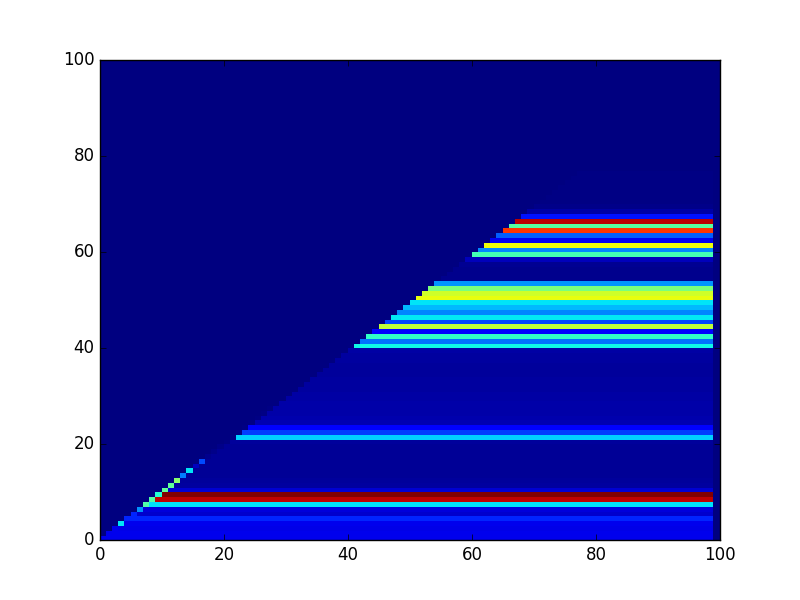
\includegraphics[width=12.6cm,height=8cm]{"C:/Users/Torstein/Documents/UiO/Mat1110/Python programmer"/Oblig2_4e.png}
Ikke kjør dette programmet for det tar ekstremt lang tid å kjøre. Tror ikke dette er riktig svar siden det krever at vi skal sjekke over en million punkter, men skjønner ikke helt oppgaven hvis det er feil. Kjørte programmet med $K = 100$ og da fikk jeg bildet over.
				\end{flushleft}
\end{document}